
\section{Empirical Evidences}



\subsection{{Forecasting Comovement}}
\label{Forecasting Comovement}

	Figure \ref{mcorr50} plots stock return comovement for different levels of common ownership, measured by MFCAP.  Higher levels of common	ownership between two firms seem to be associated with stronger correlation in their stock returns. In order to study the impact of common ownership on stock return comovement, we empirically estimate the effect of lagged measures of common ownership on stock return comovement. 
	\begin{figure}[htbp]
	\centering  
	\centering
	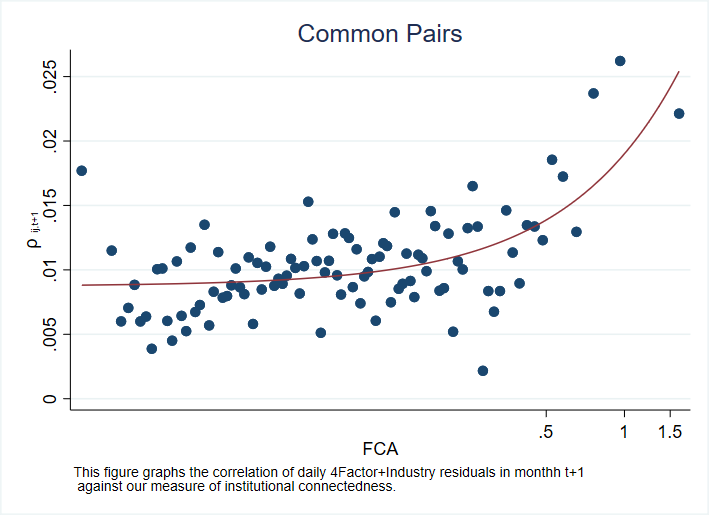
\includegraphics[width=0.7\linewidth]{"Output/mcorr50.eps"} 
	\caption{Comovement for different level of common ownership }
	\label{mcorr50}
\end{figure}
	
	We estimate a series of cross-sectional regression models in which the dependent variable is within-month realized correlation ($\rho_{i,j,t+1}$) of abnormal returns of stock pairs. As explained in section \ref{comovement}, abnormal returns are the daily residuals of a model consisting of Fama-French four factors plus industry returns. The main independent vairable of interest is our measure of common ownership, $\textit{MFCAP}^*_{ij,t}$. We are also interested in the effect of being part of the same business group,  $\textit{Same Group}_{ij} $, on stock return comovement.
		\begin{equation}
\begin{split}
\rho_{ij,t+1} = & \text{ 	}\beta_0 + \beta_1* \text{FCA}^*_{ij,t} + \beta_2* \text{SameGroup}_{ij} \\
 &	+\beta_3* \text{FCA}^*_{ij,t} \times \text{SameGroup}_{ij}   \\
  & + \sum_{k=1} ^{n} \alpha_k*\text{Control}_{ij,t} + \varepsilon_{ij,t+1}
\end{split}
\label{model1}
\end{equation}

	
	To mitigate the autocorrelation problem, we estimate the cross sectional regressions each month and report the time-series average as in \cite{FamaMacBeth}. We then use  \cite{newey1987hypothesis} to calculate standard errors of our Fama-MacBeth regressions by taking into account autocorrelation in the time series of cross-sectional estimates for four lags \textit{ paranthesis is not necessary }($ 4(71/100)^{\frac{2}{9}} = 3.71 \sim 4 $).
	
	
The estimated results are presented in panel table \ref{re1}. Panel \subref{mresult2part1} reports results from forcasting cross-sectional variation in comovement.
In the two first columns, we estimate a simplified version of equation \ref{model1} with only common ownership measure ($ MFCAP^*_{i,j}$) to investigate the relationship between common ownership and comovement. In the first column, we estimate the model without control variables. Recall that our control variables are \textit{Same Industry}, \textit{Same Size}, \textit{Same Book to Market}, and \textit{Cross-Ownership}. The \textit{Same Size} and the \textit{Same Book to Market} are normalized to have a standard deviation of one and are transformed so that higher values indicate greater style similarity. We find that $ MFCAP^*_{i,j}$ is significant with a coefficient of $0.00325$ and a t-statistics of $4.97$ in the presence of control variables. 
		
		
		In Columns 3 and 4 of that table, we use another simplified version of equation \ref{model1}, with only Same Group. The estimated coefficient in this specification, Same Group is highly statistically significant, with a coefficient of   $0.0246$ and a t-statistics of $8.2$. According to the results, there is a significant difference in the impact of the same business groups and the common ownership. 
		
		In the fifth specification of panel \subref{mresult2part1}, we use both \textit{Same Group}  and $\text{MFCAP}^*_{ij,t}$ as a forecasting variable. In this specification, only  \textit{Same Group} has a significant effect on our estimation. It suggests that common ownership affects the firms through the same business group. In the last column, we control for pairs size type (Pairs is large or small if both firms are large or small . If one firm is large and the other is small, we call it a hybrid.), which seems important for investigating firms' comovement.	\cite{AntonPolk} restrict their analysis to large firms, but we do not restrict our investigation, and our result may be driven due to this difference. Estimation result shows that by controlling pairs' type \textit{Same Group} significantly increases comovement rather than common ownership.
	
	In panel \subref{mresult2part1}, we report estimation with our control variables. Recall that these control variables (Except CrossOwnership and dummy variables) are normalized to have a standard deviation of one and are transformed so that higher values indicate greater style similarity. The presence of two firms in the same industry, SameIndustry, forecasts an abnormal return correlation with a statistically significant coefficient of 0.021 (t-statistic of6.68). The similarity in book-to-market has an effect as the coefficient on SameBM is 0.022 (t-statistic of 6.34). Of course, one should consider the fact that we are already controlling for exposure to the book-to-market factor, HML, and industry return by forecasting the correlation of four-factor plus industry residuals rather than the correlation of raw returns. We find that stocks with a similar size; the coefficient on SameSize is 0.014 (t-statistic of 4). 
	
	
	
	In panel \subref{mresult2part2}, we examine the effect of common ownership in the business groups. In the two first columns, we restrict our investigation to two sub-samples. In the first one, we run our model for the pairs in the same business group and others who do not belong to the same one. It provides evidence that common ownership only matters for the pairs in the same business groups.	
	Now for the main analysis, we include the interaction of \textit{Same Group} and $\text{MFCA}^*_{ij,t}$. We include the business group fixed effects to capture the group's characteristics for the last column. In these specifications, the economic effect of \textit{Same Group} is not significant anymore, which cannot be reliable due to the high correlation of interaction term with \textit{Same Group}($\rho = 0.75$). These results aver that $\text{MFCA}^*_{ij,t}$ has a larger effect for the pairs in the same business group. It puts forward that the \textit{Same Group}  affects comovement through indirect common ownership, which arises due to the same ultimate owner. 
	
	
	
	
		\captionsetup[subtable]{labelformat=parens,font=small}
			\renewcommand{\thesubtable}{\Alph{subtable}}
\newgeometry{top=20mm, bottom=30mm}
{\begin{table}[p]
		\centering
		\centerfloat
		\caption{Connected Comovement\\ \small
		This table reports \cite{FamaMacBeth} estimates of monthly cross-sectional regressions forecasting the correlation of daily \cite{fama1993differences}–\cite{Carhart4Factor} plus industry residuals in month t + 1 for the sample of stocks defined in Table \ref{st1}. The independent variables are updated monthly include our measure of institutional connectedness, the number of equal percents held block-holder, $\text{MFCA}^*_{ij,t}$, and a series of controls at time t. We measure the negative of the absolute value of the difference in size and book-to-market ratio (BE/ME) percentile ranking across the two stocks in the pair (SameSize, and SameBM, respectively). All independent variables, excluding dummy variables, are then rank-transformed and normalized to have a unit standard deviation. We calculate \cite{newey1987hypothesis} standard errors (four lags) of the \cite{FamaMacBeth} estimates that take into account autocorrelation in the cross-sectional slopes. We report the associated t-statistics in parentheses.
		We report estimates of regressions using variables to investigate the effect of common ownership and business group in Panel \subref{mresult2part1}. Panel \subref{mresult2part2} shows the estimation result for investigating the effect of common ownership in the business groups. }
		\label{re1}
		\subcaption{The main analysis}
		\label{mresult2part1}
		\resizebox{0.9\textwidth}{!}{
				{{
\def\sym#1{\ifmmode^{#1}\else\(^{#1}\)\fi}
\begin{tabular}{l*{6}{c}}
\hline\hline
                    &\multicolumn{6}{c}{Dependent Variable:  Future Pairs's Comovement}                                                                 \\\cmidrule(lr){2-7}
                    &\multicolumn{1}{c}{(1)}         &\multicolumn{1}{c}{(2)}         &\multicolumn{1}{c}{(3)}         &\multicolumn{1}{c}{(4)}         &\multicolumn{1}{c}{(5)}         &\multicolumn{1}{c}{(6)}         \\
\hline
$ \text{MFCAP*} $   &     0.00600\sym{***}&     0.00328\sym{***}&                     &                     &     0.00104         &    0.000929         \\
                    &      (8.10)         &      (4.87)         &                     &                     &      (1.68)         &      (1.53)         \\
[1em]
SameGroup           &                     &                     &      0.0358\sym{***}&      0.0254\sym{***}&      0.0242\sym{***}&      0.0219\sym{***}\\
                    &                     &                     &      (9.99)         &      (8.45)         &      (8.21)         &      (7.02)         \\
[1em]
SameIndustry        &                     &      0.0267\sym{***}&                     &      0.0216\sym{***}&      0.0212\sym{***}&      0.0215\sym{***}\\
                    &                     &      (7.39)         &                     &      (6.81)         &      (6.72)         &      (6.80)         \\
[1em]
SameBM              &                     &      0.0224\sym{***}&                     &      0.0213\sym{***}&      0.0214\sym{***}&      0.0199\sym{***}\\
                    &                     &      (6.41)         &                     &      (6.09)         &      (6.16)         &      (5.77)         \\
[1em]
SameSize            &                     &      0.0123\sym{**} &                     &      0.0143\sym{***}&      0.0138\sym{***}&      0.0254\sym{***}\\
                    &                     &      (3.24)         &                     &      (3.85)         &      (3.71)         &      (5.56)         \\
[1em]
CrossOwnership      &                     &      0.0600\sym{***}&                     &      0.0300\sym{*}  &      0.0316\sym{*}  &      0.0377\sym{**} \\
                    &                     &      (5.50)         &                     &      (2.36)         &      (2.48)         &      (2.93)         \\
[1em]
Constant            &      0.0142\sym{***}&      0.0204\sym{***}&      0.0103\sym{***}&      0.0187\sym{***}&      0.0188\sym{***}&      0.0280\sym{***}\\
                    &     (12.80)         &      (8.91)         &      (9.42)         &      (7.99)         &      (8.04)         &      (9.43)         \\
\hline
PairType Control    &          No         &          No         &          No         &          No         &          No         &         Yes         \\
Observations        &      389591         &      389591         &      389591         &      389591         &      389591         &      389591         \\
\hline\hline  \end{tabular}}
}
		}
		\bigskip
		\subcaption{Common Ownership and Business Group}
		\label{mresult2part2}
		\resizebox{0.9\textwidth}{!}{
					
						{{
\def\sym#1{\ifmmode^{#1}\else\(^{#1}\)\fi}
\begin{tabular}{l*{4}{c}}
\hline\hline
                &\multicolumn{4}{c}{Dependent Variable: Future Pairs's co-movement'}        \\\cmidrule(lr){2-5}
                &\multicolumn{1}{c}{(1)}         &\multicolumn{1}{c}{(2)}         &\multicolumn{1}{c}{(3)}         &\multicolumn{1}{c}{(4)}         \\
\hline
$ \text{MFCAP*} $&  0.00944\sym{***}& 0.000397         & 0.000377         &-0.0000113         \\
                &   (7.24)         &   (0.68)         &   (0.65)         &  (-0.02)         \\
[1em]
Same Group      &                  &                  &  0.00624\sym{**} &  0.00549\sym{*}  \\
                &                  &                  &   (2.81)         &   (2.27)         \\
[1em]
 $ (\text{MFCAP}^*) \times {\text{SameGroup} }  $ &                  &                  &  0.00992\sym{***}&   0.0107\sym{***}\\
                &                  &                  &   (6.49)         &   (6.97)         \\
\hline
Observations    &    58337         &  1607659         &  1665996         &  1665996         \\
Sub-sample      &SameGroup         &   Others         &      All         &      All         \\
Group Effect    &       No         &       No         &       No         &      Yes         \\
Controls        &      Yes         &      Yes         &      Yes         &      Yes         \\
$ R^2 $         &   0.0112         & 0.000577         & 0.000898         &  0.00575         \\
\hline\hline
\multicolumn{5}{l}{\footnotesize \textit{t} statistics in parentheses}\\
\multicolumn{5}{l}{\footnotesize \sym{*} \(p<0.05\), \sym{**} \(p<0.01\), \sym{***} \(p<0.001\)}\\
\end{tabular}
}
}
					
				}
		
\end{table}}
\restoregeometry
%{\begin{table}[p]
%		\centering
%		\caption{Connected Comovement}
%		\label{mresult2part2}
%		\resizebox{1\textwidth}{!}{
%			
%				{{
\def\sym#1{\ifmmode^{#1}\else\(^{#1}\)\fi}
\begin{tabular}{l*{4}{c}}
\hline\hline
                &\multicolumn{4}{c}{Dependent Variable: Future Pairs's co-movement'}        \\\cmidrule(lr){2-5}
                &\multicolumn{1}{c}{(1)}         &\multicolumn{1}{c}{(2)}         &\multicolumn{1}{c}{(3)}         &\multicolumn{1}{c}{(4)}         \\
\hline
$ \text{MFCAP*} $&  0.00944\sym{***}& 0.000397         & 0.000377         &-0.0000113         \\
                &   (7.24)         &   (0.68)         &   (0.65)         &  (-0.02)         \\
[1em]
Same Group      &                  &                  &  0.00624\sym{**} &  0.00549\sym{*}  \\
                &                  &                  &   (2.81)         &   (2.27)         \\
[1em]
 $ (\text{MFCAP}^*) \times {\text{SameGroup} }  $ &                  &                  &  0.00992\sym{***}&   0.0107\sym{***}\\
                &                  &                  &   (6.49)         &   (6.97)         \\
\hline
Observations    &    58337         &  1607659         &  1665996         &  1665996         \\
Sub-sample      &SameGroup         &   Others         &      All         &      All         \\
Group Effect    &       No         &       No         &       No         &      Yes         \\
Controls        &      Yes         &      Yes         &      Yes         &      Yes         \\
$ R^2 $         &   0.0112         & 0.000577         & 0.000898         &  0.00575         \\
\hline\hline
\multicolumn{5}{l}{\footnotesize \textit{t} statistics in parentheses}\\
\multicolumn{5}{l}{\footnotesize \sym{*} \(p<0.05\), \sym{**} \(p<0.01\), \sym{***} \(p<0.001\)}\\
\end{tabular}
}
}
%			
%		}
%\end{table}}


		\FloatBarrier

		
		
		
		
		
		
		
		
		\subsection{{High level of common ownership}}
		
			In line with the previous estimations, figure \ref{Qmcorr5lrd} provides that a higher level of common ownership affects more on the firms' comovement. As shown in panel  \subref{measureResults} table \ref{st2}, pairs in the same business group have a higher level of common ownership than others. So, the previous results could be driven by a high level of common ownership. For detailed analysis, we restrict our sample to the higher level of common ownership, which we define as the pairs with $\text{MFCAP}_{ij,t}$ in the fourth quarter in each period. Figure \ref{Qmcorr5subsample} shows the relation between future comovement and current measurement of common ownership for that pairs. As you can see in right panel, in line with the last explanation, common ownership only affects the pairs in the same group, and common ownership without the same group will not affect pairs' comovement although for a high level of common ownership.
			
			\begin{figure}[htbp]
				\centering  
				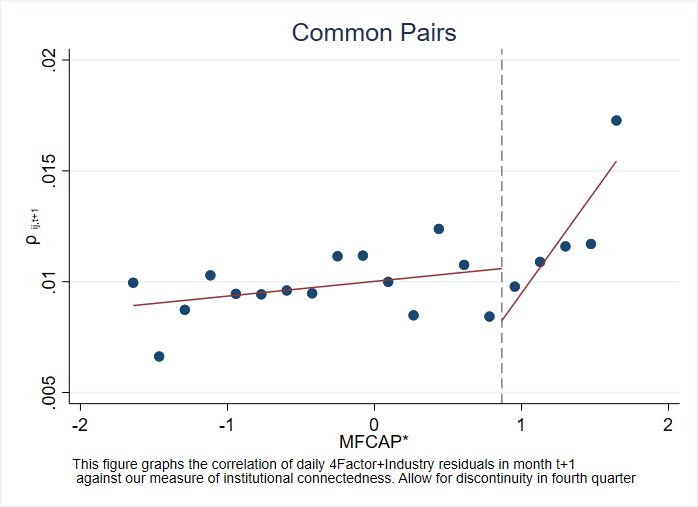
\includegraphics[width=0.65\linewidth]{"Output/Qmcorr5lrd.eps"}
				\caption{ Comovement for different level of common ownership}
				\label{Qmcorr5lrd}
			\end{figure}
			
			
						\begin{figure}[htbp]
							\centerfloat
							\resizebox{1.3\textwidth}{!}{
							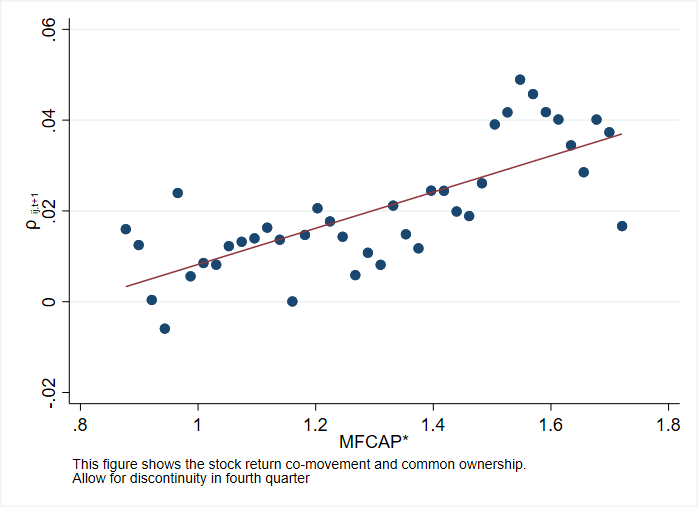
\includegraphics[width=0.55\linewidth]{"Output/Qmcorr5subsample.eps"}
							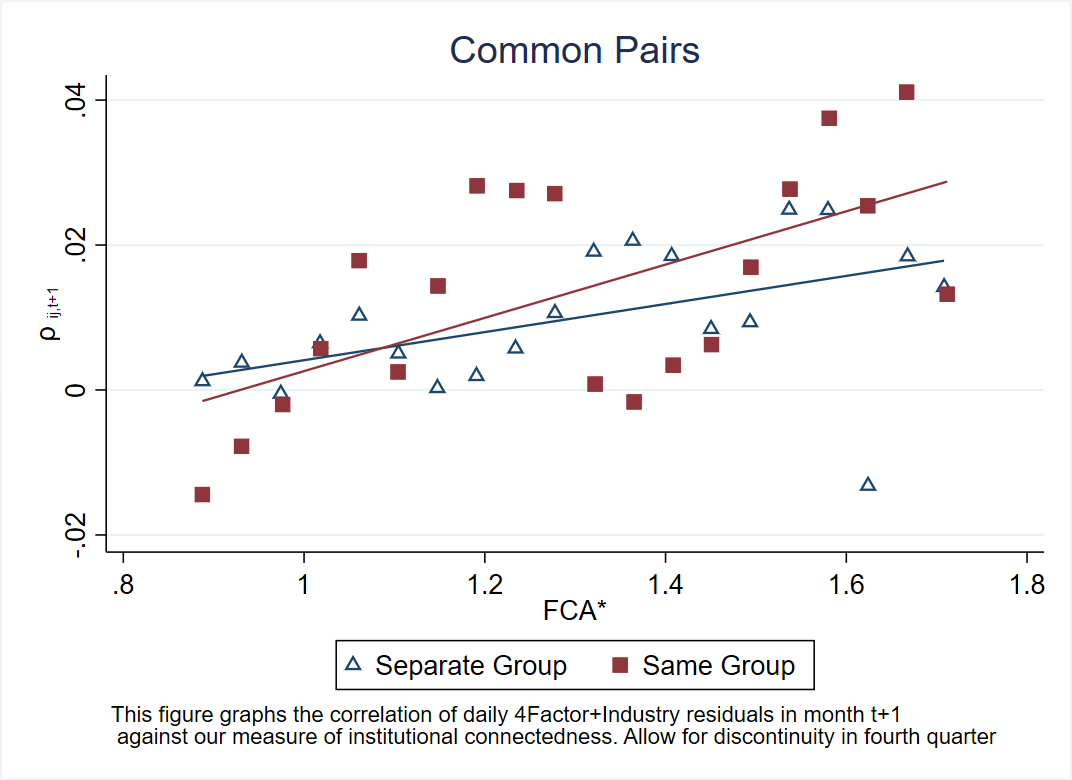
\includegraphics[width=0.55\linewidth]{"Output/Qmcorr5lrdbgsubsample.eps"}}
%							\label{Qmcorr5subsamplebg}
							\caption{Comovement for different level of common ownership for pairs in the fourth quarter}
								\label{Qmcorr5subsample}
						\end{figure}
%			\begin{figure}[htbp]
%				\centering  
%				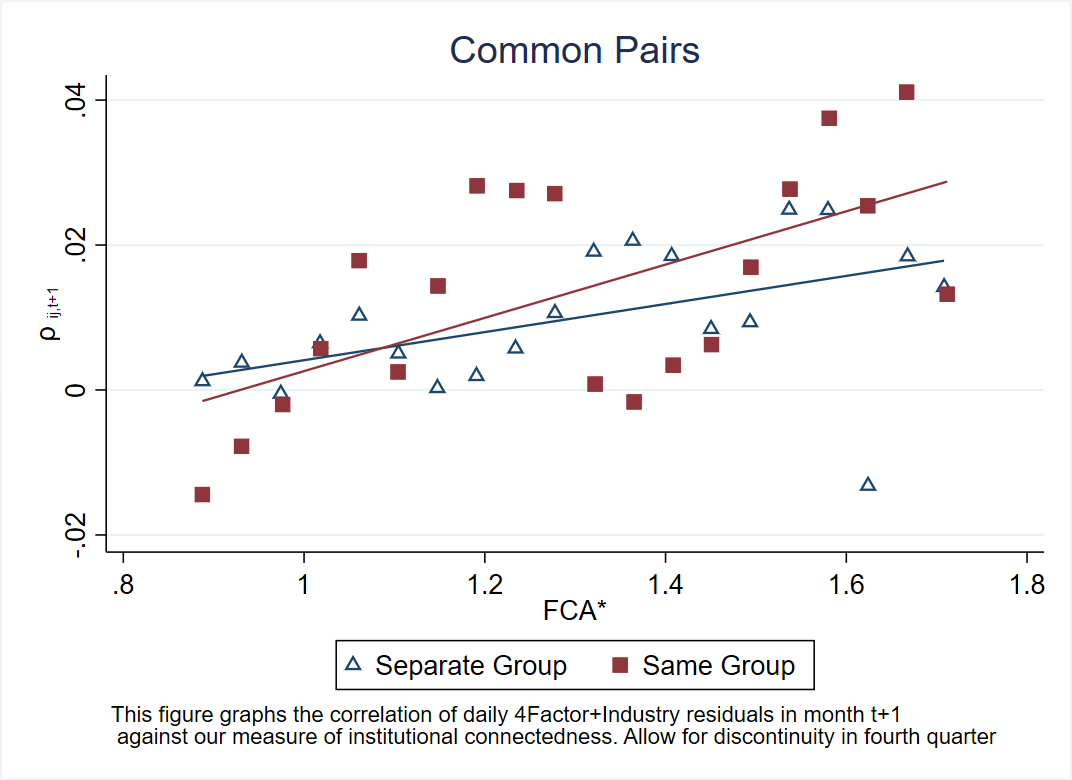
\includegraphics[width=0.65\linewidth]{"Output/Qmcorr5lrdbgsubsample.eps"}
%				\caption{Comovement for different level of common ownership for pairs in the fourth quarter}
%				\label{Qmcorr5subsamplebg}
%			\end{figure}
			
			
	
	We estimate the equation \ref{model1} with the same methodology in section \ref{Forecasting Comovement}  for the sub-sample of a high level of common ownership. Panel \subref{QTimemresult2subsample} of table \ref{re2}  reports estimations results. As expected, firms in the same business group have a high statistical and economically significant effect on forecasting future comovements. Columns three to seven confirm our prior explanations for the importance of business groups compared to common ownership in pairs with a higher level of common ownership. Pairs in the fourth quarter may have different characteristics that affect our results.  In table \ref{QarterSummary}, we summarized our control variables which shows that pairs' attributes do not look significantly different than other pairs except the presence of the pairs in the same group, which we want to examine this feature.
	
%			{\begin{table}[htbp]
%					\centering
%					\caption{High level of common ownership\\ \small
%					This table reports \cite{FamaMacBeth} estimates of monthly cross-sectional regressions forecasting the correlation of daily \cite{fama1993differences}–\cite{Carhart4Factor} plus industry residuals in month t + 1 for the pairs with the high level of common ownership. This means that our estimation is limited to the subsample of stocks defined in Table \ref{t2-2} with common ownership, which is in the fourth quarter of each period. The independent variables are updated monthly include our measure of institutional connectedness, the number of equal percents held block-holder, $\text{MFCAP}^*_{ij,t}$, and a series of controls at time t. We measure the negative of the absolute value of the difference in size and book-to-market ratio (BE/ME) percentile ranking across the two stocks in the pair (SameSize, and SameBM, respectively). All independent variables, excluding dummy variables, are then rank-transformed and normalized to have a unit standard deviation. We calculate \cite{newey1987hypothesis} standard errors (four lags) of the \cite{FamaMacBeth} estimates that take into account autocorrelation in the cross-sectional slopes. We report the associated t-statistics in parentheses. Controls not shown here are reported in the Internet Appendix.}
%					\label{QTimemresult2subsample}
%					{
%						\resizebox{\textwidth}{!}{
%						{
\def\sym#1{\ifmmode^{#1}\else\(^{#1}\)\fi}
\begin{tabular}{l*{7}{c}}
\hline\hline
                &\multicolumn{7}{c}{Dependent Variable:  Future Pairs's Comovement}                                                                  \\\cmidrule(lr){2-8}
                &\multicolumn{1}{c}{(1)}         &\multicolumn{1}{c}{(2)}         &\multicolumn{1}{c}{(3)}         &\multicolumn{1}{c}{(4)}         &\multicolumn{1}{c}{(5)}         &\multicolumn{1}{c}{(6)}         &\multicolumn{1}{c}{(7)}         \\
\hline
SameGroup       &   0.0254\sym{***}&                  &   0.0249\sym{***}&                  &                  &  0.00477         &  0.00252         \\
                &   (8.45)         &                  &   (8.21)         &                  &                  &   (1.32)         &   (0.66)         \\
[1em]
$ (\text{MFCAP} > \text{Larger than 75th Percentile}) $ &                  &  0.00660\sym{***}& 0.000777         &   0.0230\sym{***}& -0.00258\sym{*}  & -0.00157         &-0.000513         \\
                &                  &   (5.48)         &   (0.73)         &   (7.09)         &  (-2.00)         &  (-1.29)         &  (-0.46)         \\
[1em]
 $ (\text{MFCAP} > Q3[\text{MFCAP}]) \times {\text{SameGroup}} $ &                  &                  &                  &                  &                  &   0.0248\sym{***}&   0.0237\sym{***}\\
                &                  &                  &                  &                  &                  &   (7.24)         &   (7.34)         \\
\hline
Sub-sample      &      All         &      All         &      All         &SameGroup         &   Others         &      All         &      All         \\
Controls        &      Yes         &      Yes         &      Yes         &      Yes         &      Yes         &      Yes         &      Yes         \\
Business Group FE&       No         &       No         &       No         &       No         &       No         &       No         &      Yes         \\
Observations    &   389591         &   389591         &   389591         &    47076         &   342515         &   389591         &   389591         \\
\hline\hline
\multicolumn{8}{l}{\footnotesize \textit{t} statistics in parentheses}\\
\multicolumn{8}{l}{\footnotesize \sym{*} \(p<0.05\), \sym{**} \(p<0.01\), \sym{***} \(p<0.001\)}\\
\end{tabular}
}

%						}
%					}
%			\end{table}}
			
%			\begin{figure}[htbp]
%				\centering  
%				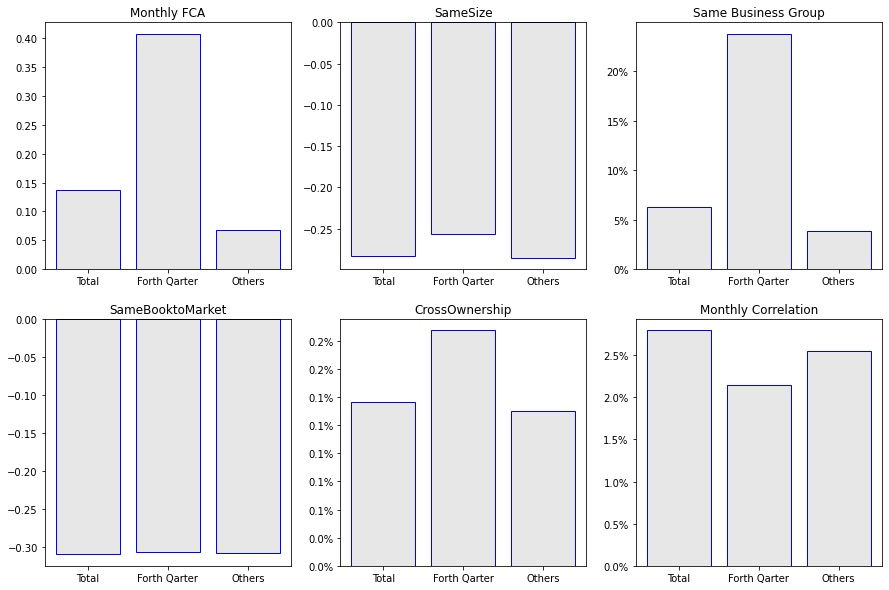
\includegraphics[width=1\linewidth]{"Output/QarterSummary.eps"}
%				\caption{Pairs' characteristics for the pairs with high level of common ownership}
%				\label{QarterSummary}
%			\end{figure}
		

				
				
				\FloatBarrier
				
				\subsection{All Pairs}
				
We restrict our investigations to firms with at least one common owner in the former analyses. By this analysis, we cannot separate the effect of the business group and common ownership; both of them can affect comovement. Furthermore, this restriction limits our result to commonly held firms, but if belonging to the same business group can increase stocks' comovement, it would affect all the firms in the same business groups. 	So, we extend our investigations by constructing all the pairs in the market to separate the effect of direct common ownership and business group and solve the mentioned problems. 
	
	For this purpose, we include stocks in one pair if they have at least two months in common. By this definition, we do not restrict our investigation to commonly held stocks and set $\text{MFCA}_{ij,t}$ to zero for a pair without any common owner. Controls are defined as before, and we use equation \ref{model1} by the same methodology as used in section \ref{Forecasting Comovement}.
	
	Panel \subref{AllPairs} table \ref{re2} reports results of estimations. These results suggest that pairs in the same group comove more than stocks not in the same group. In addition, pairs with common ownership common do not comove greater than others. In column three, we use variables of common ownership and the same business group together. Results supported our previous explanation of table \ref{re1}. The \textit{Same Group} is critical for forecasting future comovement, and common ownership matters for the pairs in the same business group.
					
%					{\begin{table}[htbp]
%							%	\centering
%							
%							\caption{Non-connected Comovement\\ \small
%							This table reports \cite{FamaMacBeth} estimates of monthly cross-sectional regressions forecasting the correlation of daily \cite{fama1993differences}–\cite{Carhart4Factor} plus industry residuals in month t + 1 for all the pairs in the market. This means that our estimation is extended to the pairs with stocks that have at least two months in common and set $\text{MFCA}_{ij,t}$ to zero for a pair without any common owner. The independent variables are updated monthly include our measure of institutional connectedness, the number of equal percents held block-holder, $\text{MFCA}^*_{ij,t}$, and a series of controls at time t. We measure the negative of the absolute value of the difference in size and book-to-market ratio (BE/ME) percentile ranking across the two stocks in the pair (SameSize, and SameBM, respectively). All independent variables, excluding dummy variables, are rank-transformed and normalized to have a unit standard deviation. We calculate \cite{newey1987hypothesis} standard errors (four lags) of the \cite{FamaMacBeth} estimates that take into account autocorrelation in the cross-sectional slopes. We report the associated t-statistics in parentheses. Controls not shown here are reported in the Internet Appendix.}			
%							\label{AllPairs}				
%							\resizebox{1\textwidth}{!}{
%									{	{
\def\sym#1{\ifmmode^{#1}\else\(^{#1}\)\fi}
\begin{tabular}{l*{7}{c}}
\hline\hline
                &\multicolumn{7}{c}{Dependent Variable: Future Pairs' co-movement}                                                                   \\\cmidrule(lr){2-8}
                &\multicolumn{1}{c}{(1)}         &\multicolumn{1}{c}{(2)}         &\multicolumn{1}{c}{(3)}         &\multicolumn{1}{c}{(4)}         &\multicolumn{1}{c}{(5)}         &\multicolumn{1}{c}{(6)}         &\multicolumn{1}{c}{(7)}         \\
\hline
SameGroup       &   0.0156\sym{***}&                  &   0.0158\sym{***}&                  &                  &   0.0138\sym{***}&   0.0131\sym{***}\\
                &   (9.84)         &                  &  (10.22)         &                  &                  &   (8.27)         &   (7.68)         \\
[1em]
$ \text{MFCAP*}  $&                  &-0.0000723         &-0.000277         &  0.00169         &-0.000322\sym{*}  &-0.000390\sym{**} &-0.000427\sym{*}  \\
                &                  &  (-0.44)         &  (-1.80)         &   (1.42)         &  (-2.19)         &  (-2.70)         &  (-2.29)         \\
[1em]
 $ (\text{MFCAP}^*) \times {\text{SameGroup} }  $ &                  &                  &                  &                  &                  &  0.00313\sym{**} &  0.00364\sym{**} \\
                &                  &                  &                  &                  &                  &   (2.80)         &   (3.34)         \\
\hline
Controls        &      Yes         &      Yes         &      Yes         &      Yes         &      Yes         &      Yes         &      Yes         \\
Sub-Sample      &    Total         &    Total         &    Total         &SameGroups         &   Others         &    Total         &    Total         \\
Business Group FE&       No         &       No         &       No         &       No         &       No         &       No         &      Yes         \\
Observations    &  6018646         &  6018646         &  6018646         &   114526         &  5904120         &  6018646         &  6018646         \\
\hline\hline
\multicolumn{8}{l}{\footnotesize \textit{t} statistics in parentheses}\\
\multicolumn{8}{l}{\footnotesize \sym{*} \(p<0.05\), \sym{**} \(p<0.01\), \sym{***} \(p<0.001\)}\\
\end{tabular}
}

%									}
%							}
%					\end{table}}
					
				
					
					
%					
%					In conclusion , these results show that same business group is more important than common ownership. In fact, when we talk about the presence of two stocks in the same business group, we talk about a high level of invisible common ownership between two stocks that we cannot measure that by mutual stockholders.
					
{\begin{table}[htbp]
		\centerfloat
			\caption{Connected Comovement\\ \small
				Panel \subref{QTimemresult2subsample} represents the estimates of monthly cross-sectional regressions forecasting the comovement for the high level of common ownership. This means that our estimation is limited to the subsample of stocks defined in Table \ref{st1} with common ownership, which is in the fourth quarter of each period. Panel \subref{AllPairs} shows the results for the estimation of that feature for all the pairs in the market, which means that the pairs with stocks that have at least two months in common and set $\text{MFCA}_{ij,t}$ to zero for a pair without any common owner. Other methods and definitions of variables are as the table \ref{re1}.  }
				\label{re2}
		\subcaption{High level of Common Ownership}
						\label{QTimemresult2subsample}
						{
							\resizebox{\textwidth}{!}{
							{
\def\sym#1{\ifmmode^{#1}\else\(^{#1}\)\fi}
\begin{tabular}{l*{7}{c}}
\hline\hline
                &\multicolumn{7}{c}{Dependent Variable:  Future Pairs's Comovement}                                                                  \\\cmidrule(lr){2-8}
                &\multicolumn{1}{c}{(1)}         &\multicolumn{1}{c}{(2)}         &\multicolumn{1}{c}{(3)}         &\multicolumn{1}{c}{(4)}         &\multicolumn{1}{c}{(5)}         &\multicolumn{1}{c}{(6)}         &\multicolumn{1}{c}{(7)}         \\
\hline
SameGroup       &   0.0254\sym{***}&                  &   0.0249\sym{***}&                  &                  &  0.00477         &  0.00252         \\
                &   (8.45)         &                  &   (8.21)         &                  &                  &   (1.32)         &   (0.66)         \\
[1em]
$ (\text{MFCAP} > \text{Larger than 75th Percentile}) $ &                  &  0.00660\sym{***}& 0.000777         &   0.0230\sym{***}& -0.00258\sym{*}  & -0.00157         &-0.000513         \\
                &                  &   (5.48)         &   (0.73)         &   (7.09)         &  (-2.00)         &  (-1.29)         &  (-0.46)         \\
[1em]
 $ (\text{MFCAP} > Q3[\text{MFCAP}]) \times {\text{SameGroup}} $ &                  &                  &                  &                  &                  &   0.0248\sym{***}&   0.0237\sym{***}\\
                &                  &                  &                  &                  &                  &   (7.24)         &   (7.34)         \\
\hline
Sub-sample      &      All         &      All         &      All         &SameGroup         &   Others         &      All         &      All         \\
Controls        &      Yes         &      Yes         &      Yes         &      Yes         &      Yes         &      Yes         &      Yes         \\
Business Group FE&       No         &       No         &       No         &       No         &       No         &       No         &      Yes         \\
Observations    &   389591         &   389591         &   389591         &    47076         &   342515         &   389591         &   389591         \\
\hline\hline
\multicolumn{8}{l}{\footnotesize \textit{t} statistics in parentheses}\\
\multicolumn{8}{l}{\footnotesize \sym{*} \(p<0.05\), \sym{**} \(p<0.01\), \sym{***} \(p<0.001\)}\\
\end{tabular}
}

							}
						}
						\bigskip
						\subcaption{All the Pairs}
\label{AllPairs}				
		\resizebox{\textwidth}{!}{
				{	{
\def\sym#1{\ifmmode^{#1}\else\(^{#1}\)\fi}
\begin{tabular}{l*{7}{c}}
\hline\hline
                &\multicolumn{7}{c}{Dependent Variable: Future Pairs' co-movement}                                                                   \\\cmidrule(lr){2-8}
                &\multicolumn{1}{c}{(1)}         &\multicolumn{1}{c}{(2)}         &\multicolumn{1}{c}{(3)}         &\multicolumn{1}{c}{(4)}         &\multicolumn{1}{c}{(5)}         &\multicolumn{1}{c}{(6)}         &\multicolumn{1}{c}{(7)}         \\
\hline
SameGroup       &   0.0156\sym{***}&                  &   0.0158\sym{***}&                  &                  &   0.0138\sym{***}&   0.0131\sym{***}\\
                &   (9.84)         &                  &  (10.22)         &                  &                  &   (8.27)         &   (7.68)         \\
[1em]
$ \text{MFCAP*}  $&                  &-0.0000723         &-0.000277         &  0.00169         &-0.000322\sym{*}  &-0.000390\sym{**} &-0.000427\sym{*}  \\
                &                  &  (-0.44)         &  (-1.80)         &   (1.42)         &  (-2.19)         &  (-2.70)         &  (-2.29)         \\
[1em]
 $ (\text{MFCAP}^*) \times {\text{SameGroup} }  $ &                  &                  &                  &                  &                  &  0.00313\sym{**} &  0.00364\sym{**} \\
                &                  &                  &                  &                  &                  &   (2.80)         &   (3.34)         \\
\hline
Controls        &      Yes         &      Yes         &      Yes         &      Yes         &      Yes         &      Yes         &      Yes         \\
Sub-Sample      &    Total         &    Total         &    Total         &SameGroups         &   Others         &    Total         &    Total         \\
Business Group FE&       No         &       No         &       No         &       No         &       No         &       No         &      Yes         \\
Observations    &  6018646         &  6018646         &  6018646         &   114526         &  5904120         &  6018646         &  6018646         \\
\hline\hline
\multicolumn{8}{l}{\footnotesize \textit{t} statistics in parentheses}\\
\multicolumn{8}{l}{\footnotesize \sym{*} \(p<0.05\), \sym{**} \(p<0.01\), \sym{***} \(p<0.001\)}\\
\end{tabular}
}

				}
		}		
		
	\end{table}}


					
					\FloatBarrier

	\captionsetup[subtable]{labelformat=empty}
